\section[Phrasal-Anchoring: Minimal Span-based CKY Parsing]{Phrasal-Anchoring: Minimal Span-Based \\CKY Parsing}
\label{sec:lex-phr:cky-based}

Let us now see our phrasal-anchoring parser for UCCA and TOP. We
introduce the transformation~(\autoref{ssec:phr:graph-ct}) used to
reduce UCCA and TOP parsing into a unified constituent tree parsing
task. Then based on the above transformation, we introduce how to do
independent factorization on phrasal-anchoring by addressing the three
main challenges in \textbf{Output
  Decomposition}~(\autoref{sssec:lex-phr:phr-output-decomposition}),
\textbf{Input Decomposition and Alignments
  Discovery}~(\autoref{sssec:lex-phr:phr-input-decomposition}), and
\textbf{Factor Modelling}, including CKY
parsing~(\autoref{ssec:phr:cky}) and span representation
~(\autoref{ssec:phr:span})


\subsection{Graph to Constituent Tree Transformation}
\label{ssec:phr:graph-ct}
Nodes in UCCA do not have node labels or node properties, but all the
nodes are anchored to the spans of the underlying sentence. However,
to have a unifed representation with previous lexical anchoring, we do
the following transformation to form a constituent tree for UCCA,
where every node has a label, which is suitable for the independent
facrtorization to map each input decompositions into the output nodes.

\subsubsection{UCCA to Consistuent Tree Transformation}
\label{sssec:phr:ucca-to-ct}
We propose to transform a graph into a constituent tree structure for
parsing, which is also used in recent work~\cite{jiang2019hlt}.
Figure~\ref{fig:ucca-to-CT} shows an example of transforming a UCCA
graph into a constituent tree. The primary transformation assigns the
original label of an edge to its child node. Then to make it
compatible with parsers for standard PennTree Bank format, we add some
auxiliary nodes such as special nonterminal nodes, \kw{TOP},
\kw{HEAD}, and special terminal nodes \kw{TOKEN} and \kw{MWE}. We
remove all the~\tquoted{remote} annotation in UCCA since the
constituent tree structure does not support reentrance.  A fully
compatible transformation should support both graph-to-tree and
tree-to-graph transformation.

In our case, to simplify the model, we remove those remote edges and
reentrance edges during training. Besides that, we also noticed that
for multiword expressions, the children of a parent node might not be
in a continuous span (\eg, discontinuous constituent), which is also
not supported by our constituent tree parser. Hence, when training the
tree parser, by reattaching the discontinuous tokens to its nearest
continuous parent nodes, we force every sub span are continuous in the
transformed trees. We leave the postprocessing to recover those
discontinuous as future work.

For inference, given an input sentence, we first use the trained
constituent tree parsing model to parse it into a tree, and then we
transform a tree back into a directed graph by assigning the edge
label as its child's node label, and deleting those auxiliary labels,
adding anchors to every remaining node.

\begin{figure}[!h]
\begin{center}
\includegraphics[width=0.90\textwidth]{dog-ucca-to-CT.pdf}
\end{center}
\caption{\label{fig:ucca-to-CT} UCCA to constituent tree transformation for [wsj\#0209013].}
\end{figure}

\subsubsection{TOP to Consistuent Tree}
\label{sssec:phr:top-to-ct}
For the hierarchical dialogue representation TOP, we also can tranform
it to a constituent tree structure. \autoref{fig:TOP-to-CT} shows the
transformation process for the utterance ``Driving directions to the
Eagles game". In TOP tree shown in the up side of the figure, the leaf
nodes are not single words as in consituent tree, and there are no
other nonterminal nodes~(such as part-of-speech tags) other than the
intents and slots nodes. Hence, we decompose the original teriminal
nodes in TOP into seperate tokens, and add a special parent node as
\texttt{TOK} to each of the ternimal token node. Finally, it forms the
constituent tree as shown in the bottom.
\begin{figure}[!h]
\begin{center}
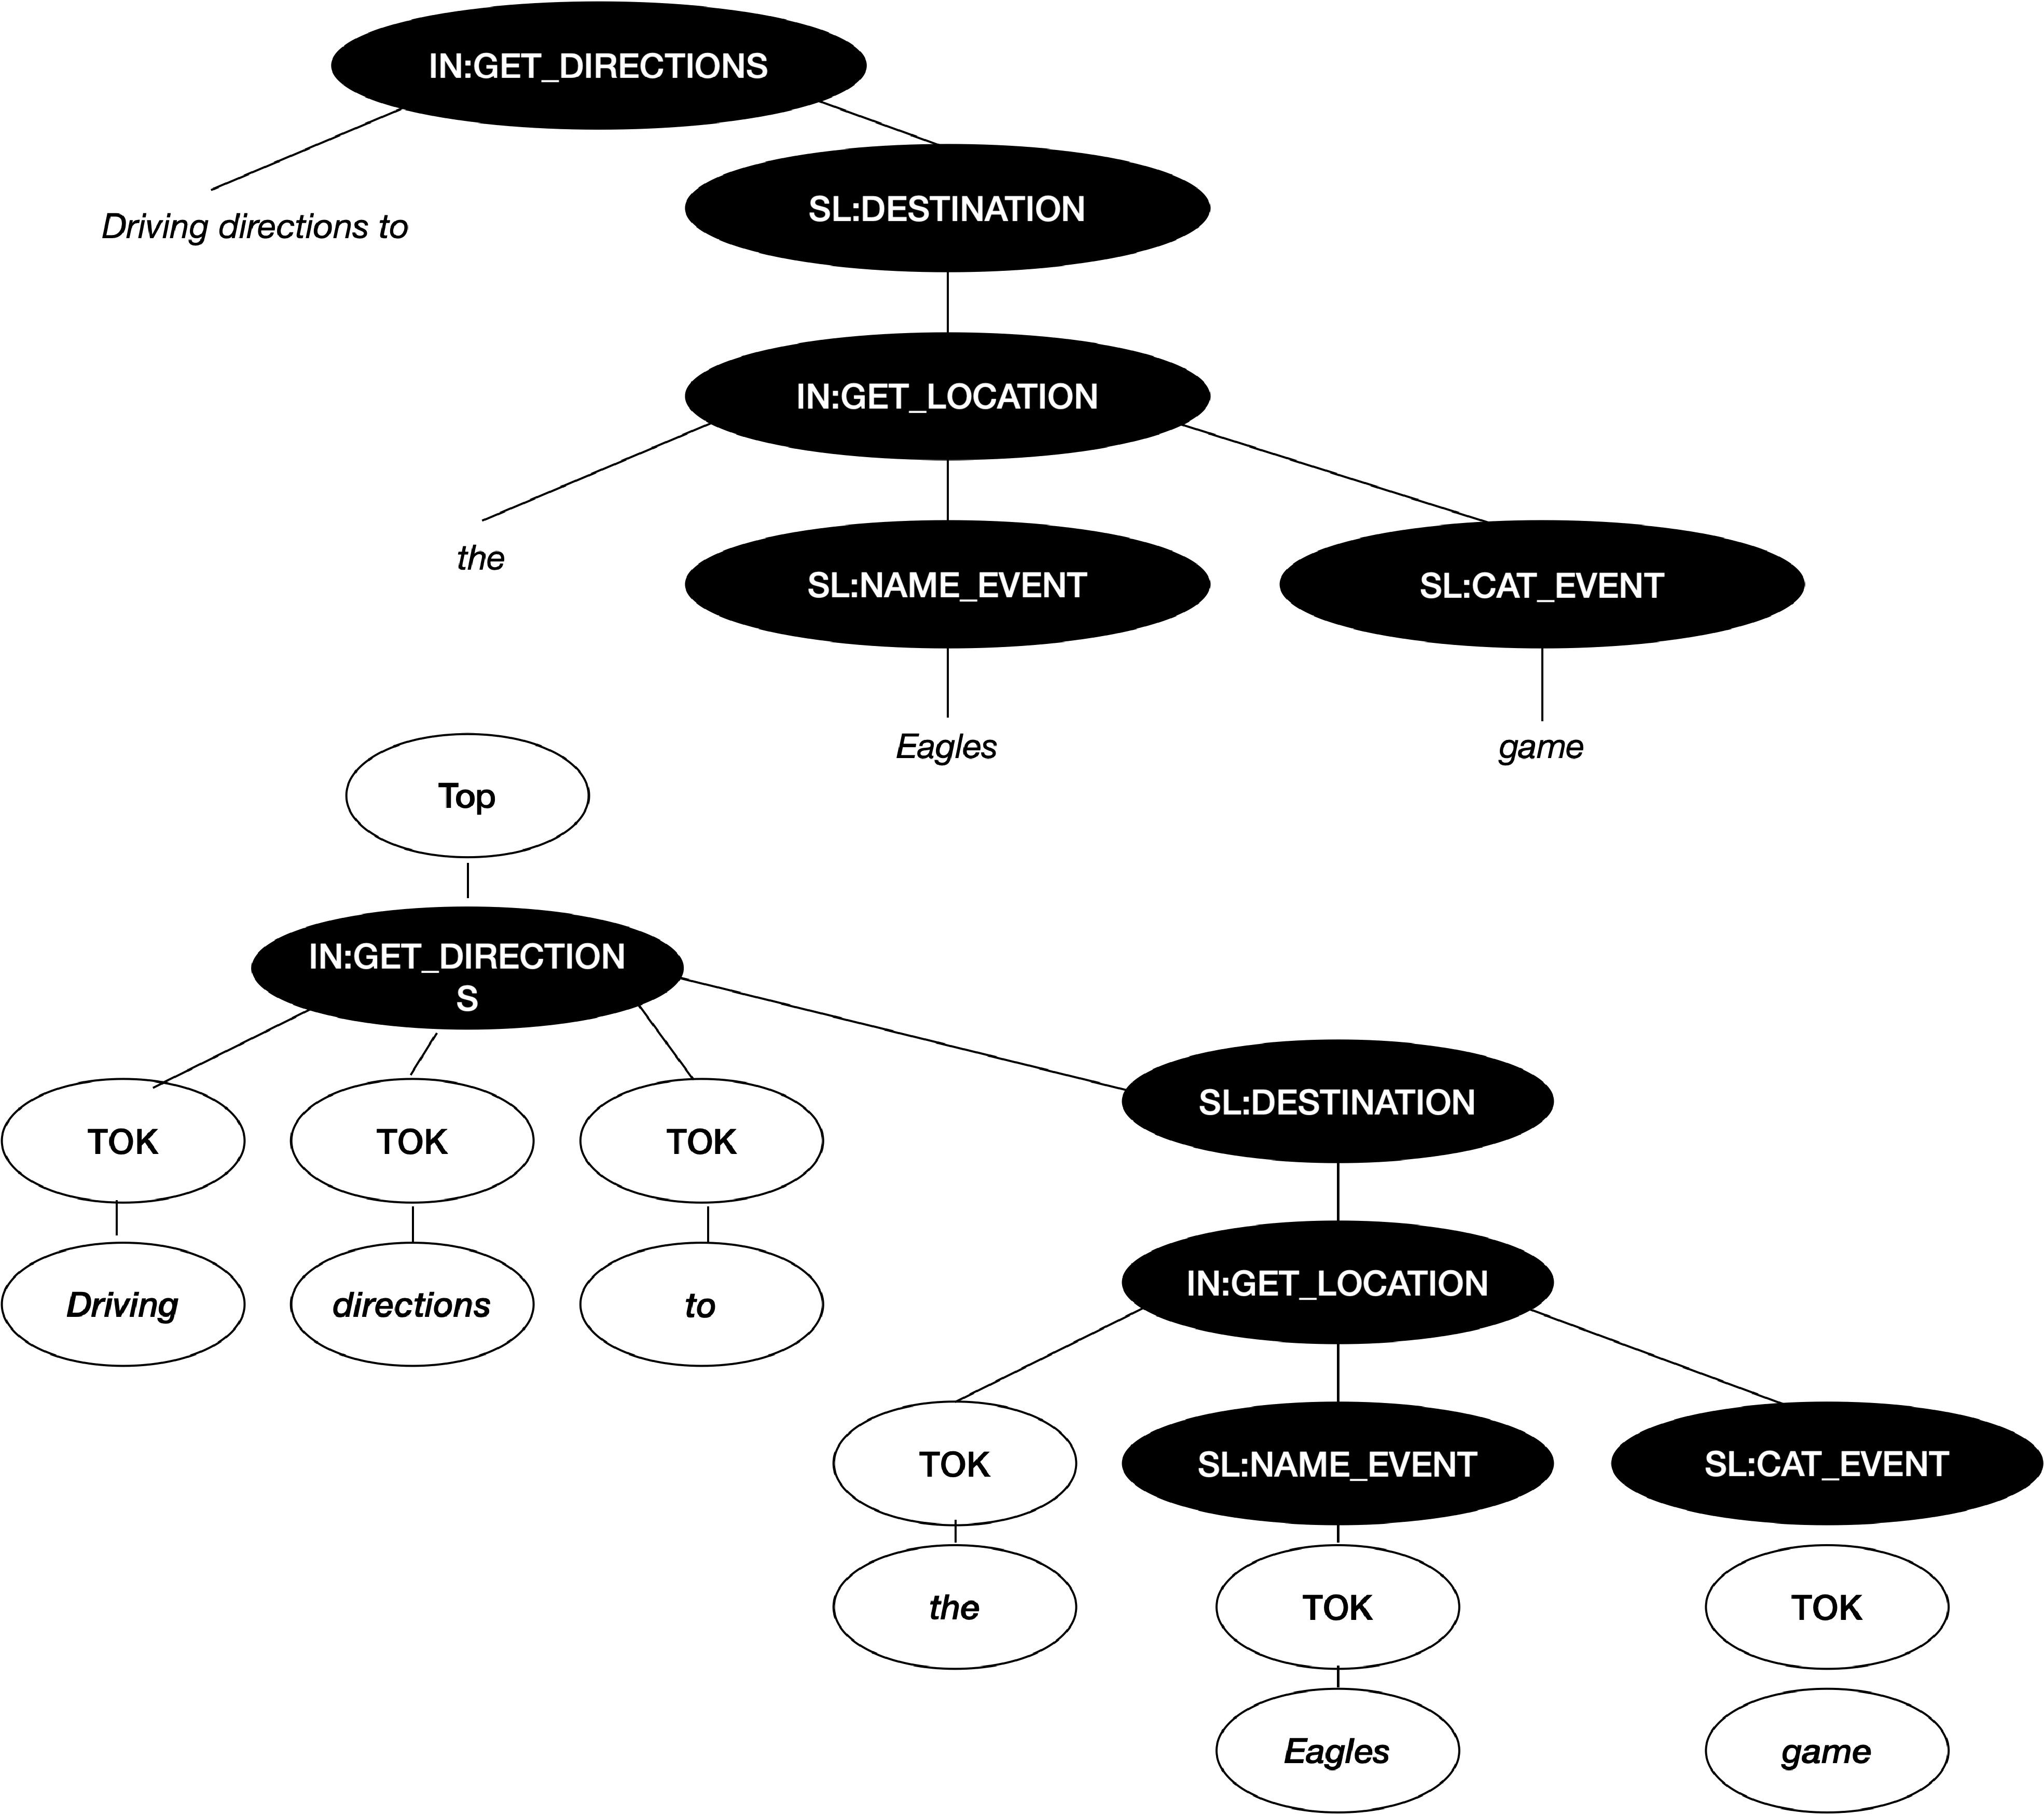
\includegraphics[width=0.90\textwidth]{TOP-to-CT.pdf}
\end{center}
\caption{\label{fig:TOP-to-CT} TOP to constituent tree transformation
  for the utterance \tquoted{Driving directions to the Eagles game.}}
\end{figure}

%%% Local Variables:
%%% mode: latex
%%% TeX-master: "../../dissertation-main.ltx"
%%% End:


\subsection{Independent Factorization on Phrasal Anchoring}
\label{ssec:lex-phr:phr-factorization-analysis}
In the following, we focus on the first two main challenge in
independent factorization: \textbf{output decomposition} and
\textbf{input decomposition} on phrasal-anchoring parsing. We leave the
\textbf{factor modelling} into the next part. We consider the same
sentence example~\dquoted{Pierre Vinken, 61 years old, will join the board as
  a nonexecutive director Nov.29.} and its corresponding UCCA graph as
shown in~\autoref{fig:bg:ucca}. We introduce the details of
independent factorization for UCCA and other pharsal-anchoring
representations.

\subsubsection{Output Decomposition}
\label{sssec:lex-phr:phr-output-decomposition}
\begin{figure}[!tbp]
  \begin{center}
  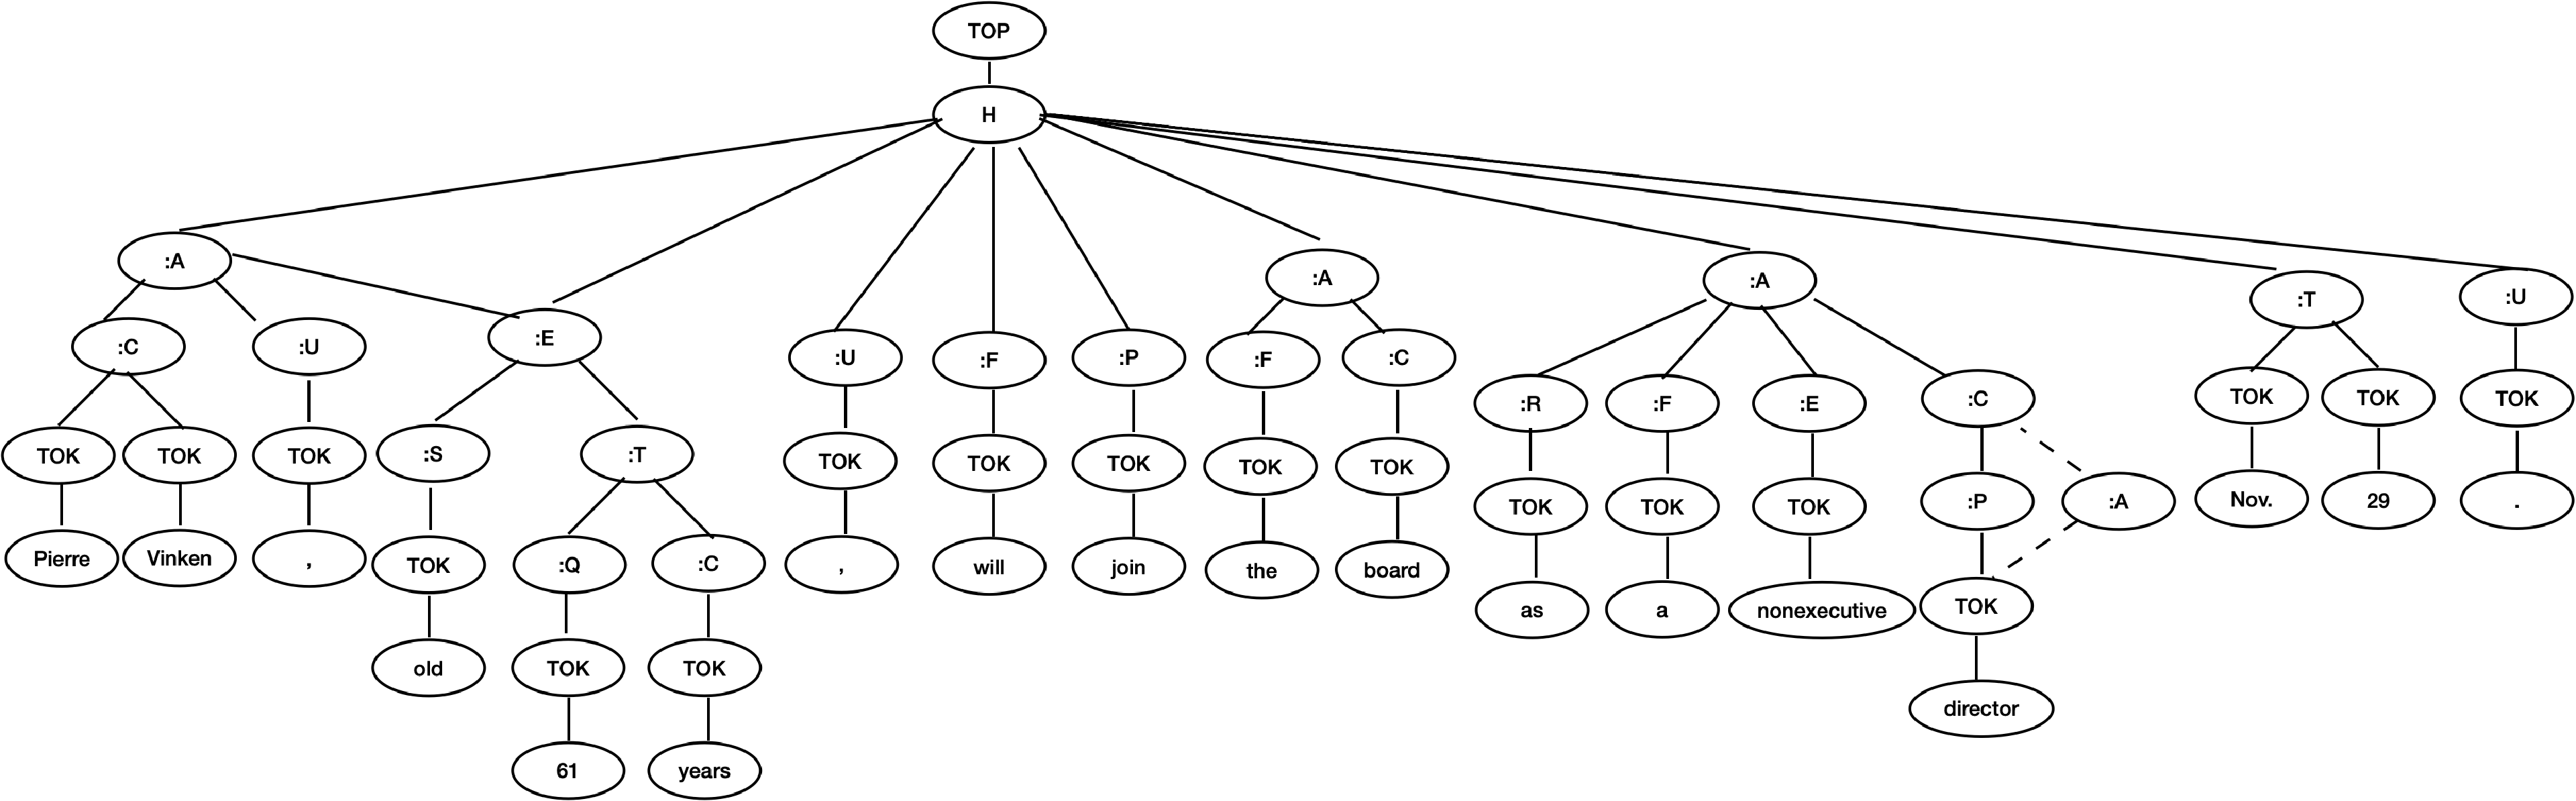
\includegraphics[width=0.98\textwidth]{pierre-ucca-decomposition.pdf}
  \end{center}
  \caption{\label{fig:lex-phr:ucca-decomposition} UCCA decomposition
    for the sentence \#20001001.}
\end{figure}
After the above transformation, as shown in the
\autoref{fig:lex-phr:ucca-decomposition} the labelled nodes in UCCA
are linked into a hierarchical structure, with edges going between
parent and child nodes. With certain exceptions~(\eg, remote edges,
the dashed line to the node \tquoted{:A} with a second parent of node
\tquoted{director}), the majority of the UCCA graphs are tree-like
structures. In this disseration, because the remote edge are rare, we
ignore all the exception to simplfy the modeling. According to the
position as well as the anchoring style, nodes in UCCA can naturally
classified into the following two types:

\begin{inparaenum}
\item \textbf{Terminal nodes} are the leaf semantic
  concepts anchored to individual lexical units in the sentence

\item \textbf{Nonterminal nodes} are usually anchored to a span with
  more than one lexical units, thus usually overlapped with the
  anchoring of terminal nodes.
\end{inparaenum}

Hence, it is natural that we can decompose the transformed UCCA tree
into two set of nodes, both of them can be produced from the
corresponding lexical units or phrases. However, more challenges
exists on how to generate the input segments that can produce those
output decompostions.

\subsubsection{Input Decomposition and Alignments Discovery}
\label{sssec:lex-phr:phr-input-decomposition}
Different from the lexical anchoring without overlapping, UCCA may
align to larger overlapped word spans which involves syntactic or
semantic pharsal structure. Further mode, the phrasal decomposition
and the alignment model is provided in training data. However, we have
no idea on how to factorize the input during inference.

In lexical anchoring, the input decomposition are handled with a
rule-based preprocessing step. However, there is no clear rules how to
decompose a sentence into a structure similar with consistuent tree
structure. Luckily, we have many previous studies on how to parse a
sentence into a constituent tree, which inspired us that we can model
the input decomposition jointly with the factor modelling part. We
leave more details of the model for joint input decomposition and
factor modeling in~\autoref{ssec:phr:cky}.

%%% Local Variables:
%%% mode: latex
%%% TeX-master: "../../dissertation-main.ltx"
%%% End:


\subsection{A Unified Span-based Model for CKY Parsing}
\label{ssec:phr:cky}
After transforming the UCCA graph into a constituent tree, we reduce
the UCCA parsing into a constituent tree parsing problem. Similar to
the previous work on UCCA constituent tree
parsing~\cite{jiang2019hlt}, we use a minimal span-based CKY parser
for constituent tree parsing.  The intuition is to use dynamic
programming to recursively split the span of a sentence recursively,
as shown in Figure~\ref{fig:ucca-to-CT}. The entire sentence can be
splitted from top to bottom until each span is a single unsplittable
tokens. For each node, we also need to assign a label. Two simplified
assumptions are made when predicting the hole tree given a
sentence. However, different with previous work, we use 8-layers with
8 heads transformer encoder, which shows better performance than LSTM
in \citet{kitaev2018constituency}.

\paragraph{Tree Factorization} In the graph-to-tree transformation, we
move the edge label to its child node. By assuming the labels for each
node are independent, we factorize the tree structure prediction as
independent span-label prediction as Equation
\ref{eq:tree_factorize}. However, this assumption does not hold for UCCA.
Please see more error analysis in \S \ref{ssec:error_breakdown}

\begin{equation}
  \label{eq:tree_factorize}
 \begin{aligned} T^{*}  & = \underset{T}{\textbf{arg\,max}} s(T)     \\ s(T)
                        & = \sum_{(i,j,l) \in T} s(i,j,l)
\end{aligned}
\end{equation}

\paragraph{CKY Parsing} By assuming the label prediction is
independent of the splitting point, we can further factorize the whole
tree as the following dynamic programming in Equation \ref{eq:tree_chart}.

\begin{equation}
  \label{eq:tree_chart}
\begin{aligned}
      s_{\text{best}}(i, i+1) & = \underset{l}{\textbf{max}} s(i,i+1, l) \\
      s_{\text{best}}(i, j) & = \underset{l}{\textbf{max}} s(i,j, l)
      \\ & + \underset{k}{\textbf{max}}[ s_{\text{best}}(i,k) +
      s_{\text{best}}(k,j) ]
\end{aligned}
\end{equation}

\subsection{Span Encoding}
\label{ssec:phr:span}

For each span $(i,j)$, we represent the span encoding vector
$v_{(i,j)} = [\vec{y_{j}} - \vec{y_{i}}] \oplus [\cev{y_{j+1}} -
\cev{y_{i+1}}] $. $\oplus$ denotes vector concatenation. Assuming a
bidirectional sentence encoder, we use the forward and backward
encodings $\vec{y_{i}}$ and $\cev{y_{i}}$ of $i_{th}$ word. Following
the previous work, and we also use the loss augmented inference
training. More details about the network
architecture are in the Section \ref{ssec:exp_setup}

%%% Local Variables:
%%% mode: latex
%%% TeX-master: "../../dissertation-main.ltx"
%%% End:
